\section{LNA Architecture}

The proposed Low Noise Amplifier (LNA) architecture employs a wideband balun topology that combines a common-gate (CG) stage and a common-source (CS) stage operating in parallel. This design is advantageous due to its capability to provide input matching, output balancing, noise cancellation, and distortion suppression~\cite{Blaakmeer2008}.

\begin{figure}[H]
    \centering
    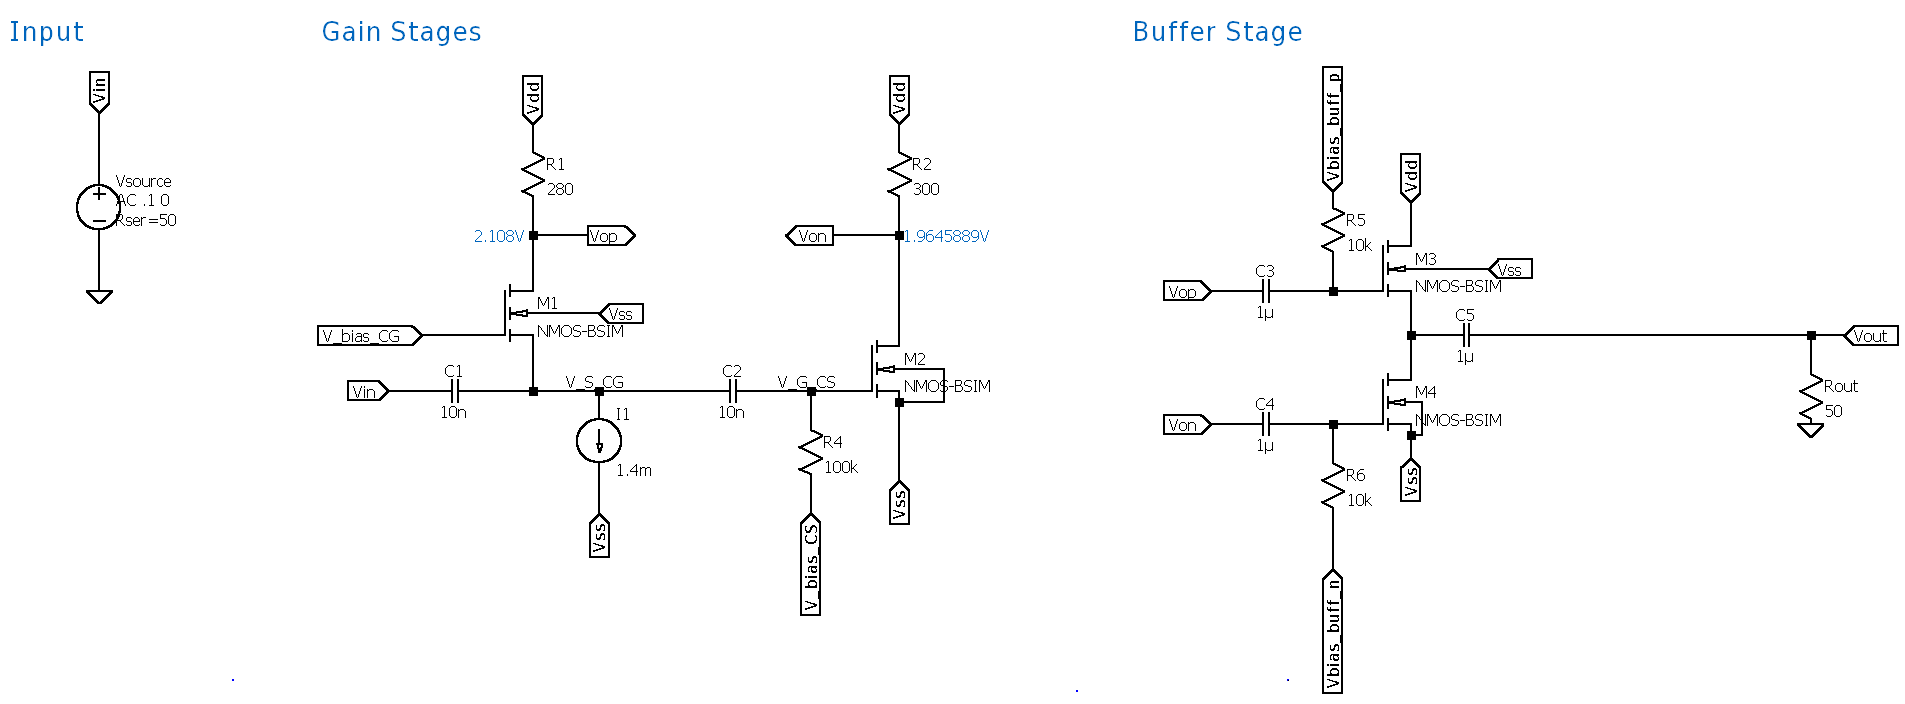
\includegraphics[width=0.8\textwidth]{Images/schem-LNA.png}
    \caption{Schematic of the proposed LNA topology.}
    \label{fig:schem-lna}
\end{figure}

As shown in Figure~\ref{fig:schem-lna}, the input signal is simultaneously amplified by the CG and CS stages. The CG stage is connected directly to the input, offering low input impedance suitable for broadband matching with a 50~\si{\ohm} source. The CS stage provides voltage amplification and operates in parallel to assist in achieving differential outputs.

The circuit produces a differential output, the positive output is taken from the drain of the CG transistor, while the negative output is taken from the drain of the CS transistor. AC coupling capacitors are placed between stages to ensure proper DC isolation.

\subsection{Common Gate Stage}

\begin{figure}[H]
    \centering
    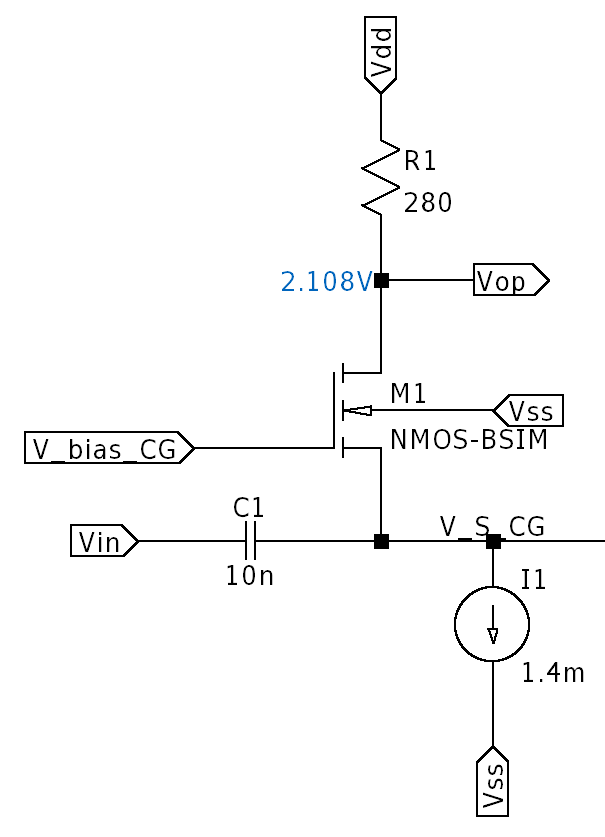
\includegraphics[width=0.3\textwidth]{Images/schem-CG.png}
    \caption{Common-Gate (CG) stage of the LNA.}
    \label{fig:schem-cg}
\end{figure}

The CG stage, illustrated in Figure~\ref{fig:schem-cg}, provides a low input impedance and enables direct broadband matching to a 50~\si{\ohm} source. This characteristic makes it ideal for RF front-end applications.

To produce differential output and achieve noise cancellation, the CG stage is complemented by a CS stage of matching gain but opposite phase. This enables the structure to perform as a balun, converting the single-ended input into a differential signal.

Noise from the CG stage, predominantly thermal, appears identically at both output nodes and is thus suppressed in the differential signal. Likewise, second-order distortion from the CG stage is canceled when the CS path has symmetric gain but opposite sign.

\subsection{Common Source Stage}

\begin{figure}[H]
    \centering
    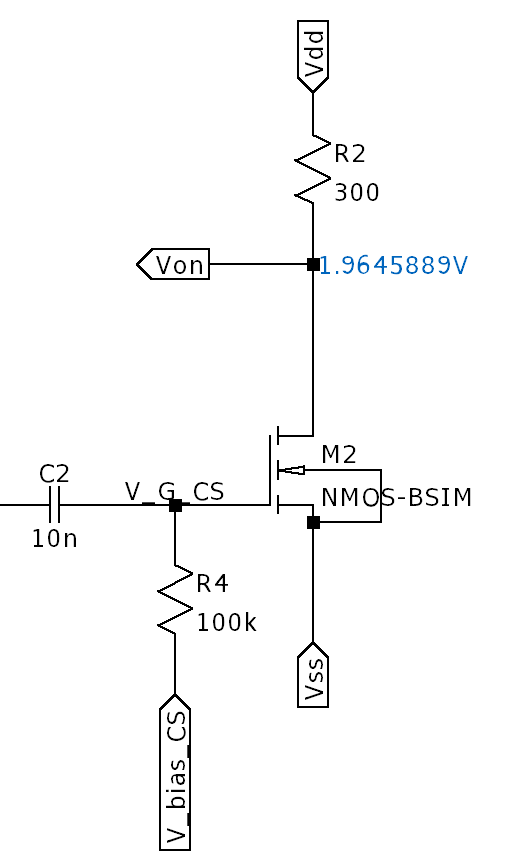
\includegraphics[width=0.3\textwidth]{Images/schem-CS.png}
    \caption{Common-Source (CS) stage of the LNA.}
    \label{fig:schem-cs}
\end{figure}

The CS stage, shown in Figure~\ref{fig:schem-cs}, offers high voltage gain and high input impedance. In this architecture, it is used in parallel with the CG stage, contributing to the differential signal and allowing cancellation of common-mode components.

The CS stage's primary contribution is not only signal gain but also linearity. As CG stage nonlinearities are canceled, the CS stage becomes the dominant source of linearity, enabling targeted optimization for dynamic range and signal integrity.

\subsection{Buffer Stage}

\begin{figure}[H]
    \centering
    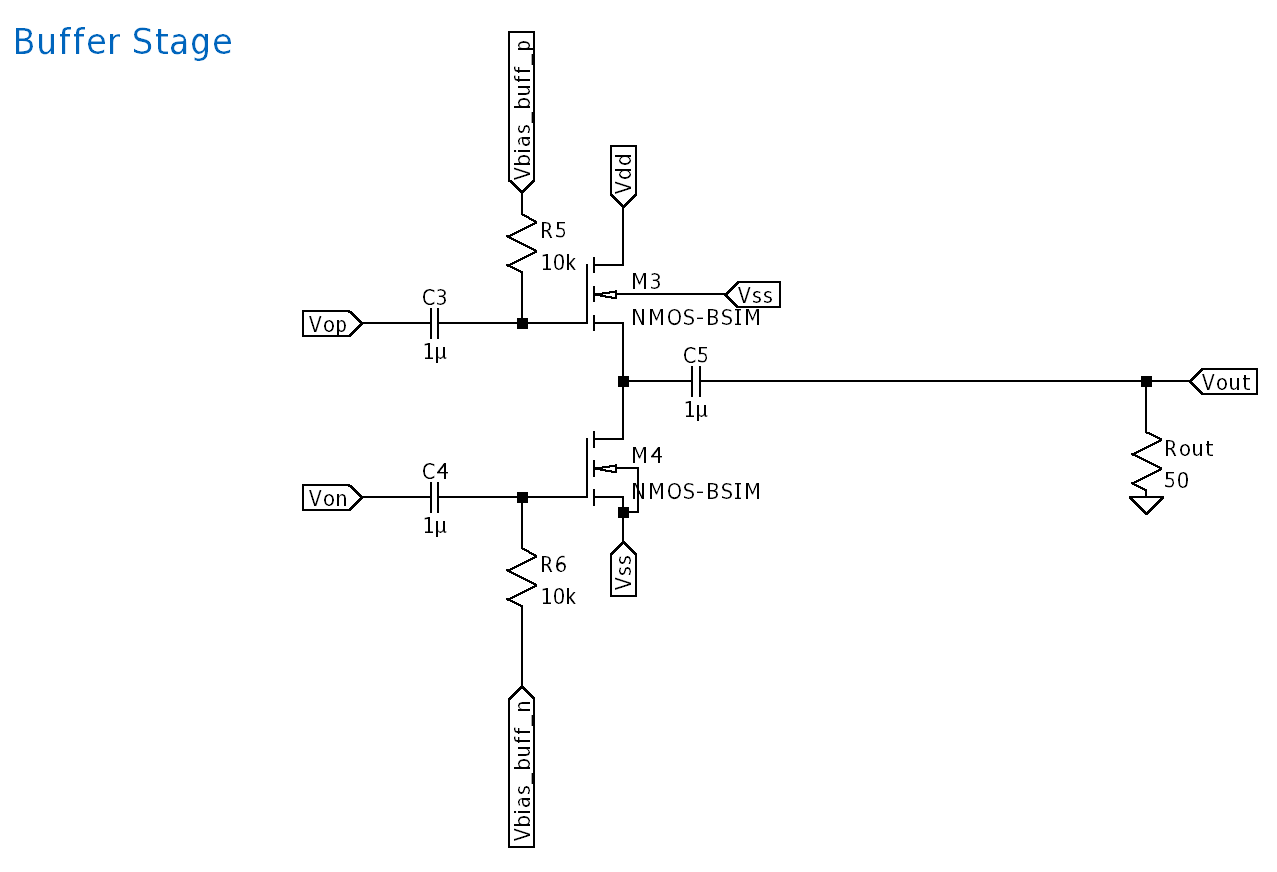
\includegraphics[width=0.6\textwidth]{Images/schem-Buffer.png}
    \caption{Output buffer stage with voltage combining.}
    \label{fig:schem-buffer}
\end{figure}

To convert the differential output into a single-ended signal and drive a 50~\si{\ohm} load, a buffer stage is added after the gain stages, in conformity with the one presented in \cite{Bastos2014}. The buffer, shown in Figure~\ref{fig:schem-buffer}, consists of transistors in both common-drain and common-source configurations, acting as a voltage combiner.

The buffer serves several purposes:
\begin{itemize}
    \item It provides low output impedance, ensuring proper matching with measurement instruments and subsequent RF stages.
    \item It isolates the gain core from external loading, preserving voltage gain and improving stability.
    \item It enables easy measurement by converting differential signals into single-ended outputs suitable for spectrum and network analyzers.
    \item It centers the output DC level around $V_{DD}/2$, enabling maximum output swing and symmetrical headroom.
\end{itemize}

The PMOS and NMOS gates are biased as follows:
\[
    V_{\text{biasn}} = V_{tn} + V_{\text{DSsat}}, \quad V_{\text{biasp}} = \frac{V_{DD}}{2} + V_{GS}
\]
where $V_{GS}$ corresponds to the gate-source voltage of the NMOS device. This ensures symmetrical operation and effective output swing.
